\chapter{Modeling the Effects of Information on Power Grids}
\label{implementationall}
In this Chapter, a framework to model, analyze, and predict 
the effects of information on social media on the 
power grid will be introduced.
First, in Section \ref{simulationframeworksection}, 
the implementation of the simulation framework will be described.
First, in Section \ref{modelsocialnetwork}, the underlying social network model
used in the simulation model is described. Second, in Section 
\ref{modelinformationdiffusion}, the algorithm used to model
the information diffusion process in the social network is 
defined. Third, in Section \ref{rulebasedpowerconsumption}, 
the rules to model the additional power consumption is explained.
Additionally, in Section \ref{parameterestimationalgo},
an parameter estimation algorithm for the estimation of 
realistic values for the simulation parameters is introduced and 
the different steps of the framework are described.

\section{Implementation of the Simulation Framework}
\label{simulationframeworksection}
There are multiple components that are necessary to model the effects of 
both true and false information on critical infrastructures
such as the power grid. The development of the simulation framework
proposed in this work can be divided into three parts. First, a model 
to describe social media networks with characteristics similar 
or equal to real social media networks must be implemented.
Second, an algorithm to model the 
propagation of information over the network needs to be defined and 
implemented. Third, rules to estimate the changes in the power consumption 
are necessary.

\subsection{Social Network Modeling Approaches}
\label{modelsocialnetwork}
Two approaches for the creation of social media network graphs 
are considered in this Thesis.

First, a real social media network can be used as an example 
social network graph model. 
It is difficult to determine which individuals
control which accounts on social media networks due to privacy reasons.
Thus, it is not possible to create a social network graph that 
shows the real state of the social media network.
Therefore, datasets can be used to avoid dealing with privacy concerns. 
There are datasets available to analyze
real social media networks, e.g. the Stanford 
Large Network Dataset Collection \cite{snapnets}.
This collection is part of the Stanford Network Analysis Project (SNAP).
In this collection, there are datasets which show the network structure
of multiple social networks such as Facebook and Twitter.
The advantage of using real social networks as reference networks
for the simulation framework is that real networks fulfill the 
characteristics of social networks, since they
are based on real data and not randomly generated. The problem
is that with this approach, all simulations use either
one or few selected social network graph models. Since 
few different graph models are used for consecutive simulations,
it cannot be determined if the simulation results are based on the 
structure of the specific social network graph or if the results 
are seasonable for other social networks, i.e. the simulation results
may not be robust. Moreover, the size of the social network graph 
cannot be changed without changing its characteristics, such as 
the clustering coefficient. Since real social network graphs tend to be 
big (for example, the Twitter social network graph provided by SNAP
contains 81306 nodes and the Facebook social network graph contains 
4039 nodes), it may not be computationally feasible to use such graphs
as reference graphs.

The other approach would be to generate a graph that is not based
on any real social network, but can be used as a reference graph.
For this, the generated graph needs to fulfill the common
characteristics of social networks.
From the information provided in Section \ref{comparison-random-graphs}, 
it is visible that the Barabási–Albert (BA) graph is the random graph 
algorithm that fulfills the characteristics of social networks most effectively.
The reason is that BA graphs are both scale-free, have the small-world
characteristic and are also clustered.
Using a random graph to model the social media network has the advantage
that each simulation can be run with an new, generated graph model. 
Thus, the simulation results can be considered more robust. 
Furthermore, different graph sizes can be 
used in the simulation by changing the number of nodes to be generated.
Thus, using random graph algorithms is computationally easier since 
real social network graphs tend to be big.
The disadvantage is that random graph models may not fulfill
all characteristics of a social network. As mentioned in 
Section \ref{comparison-random-graphs}, the BA graph
does not create graphs with a clustering coefficient that is as 
high as that of real social networks. Nonetheless, the BA graph is
a graph that is often used to model social networks.
Since the usage of random graphs allows the usage
of unique graph models for the simulation and the size of the 
graph can be changed without changing the graph characteristics, 
the random graph generation approach was used to model social networks.

A framework to create and modify the social network graph is needed to 
allow the simulation to model the information propagation
progress on the graph. \textit{NetworkX} is a 
Python package which provides various functions to model,
analyze and manipulate graph-based structures. 
The library was used in this Thesis for
the generation and modeling of the social network graph.

\subsection{Information Propagation Algorithm}
\label{modelinformationdiffusion}

There are multiple methods to model information diffusion in graph models.
In Section \ref{informationdiffsection}, three different information diffusion
model algorithms were introduced.
Both the information cascade model and the threshold model focus on the 
information diffusion process itself and not on the change in behavior
of the single entities in the system. Thus, in these two models,
entities may have two states: 
\textit{Informed} or \textit{Not Informed}.
On the other hand, epidemiological models such as the SIR model
focus on the changes of the states of the entities in the system.
Thus, it is possible to define a different behaviors in the
information diffusion progress with epidemiological models. 
In this Thesis, we are interested in both how the information
propagates and how it could be combated by using fact-checking.
This can be studied in more detail if entities can 
show different behaviors depending on what kind of information
they possess. This can only be done in epidemiological models.
Thus, an epidemiological model was chosen to model the information 
diffusion process.

Epidemiological models can be defined by differential equations.
As an example, the differential equations for the SIR and SIS 
model are shown in Table \ref{SI-table-equations}.
Nonetheless, graph-based epidemological models are also used.
In Section \ref{epidemologicalmodels}, an information 
diffusion model based on the work of \textit{Tambuscio et al.} 
\cite{sirsmodel} is introduced. It has the advantage of being 
able to model both the misinformation and fact-checking 
diffusion process in the same model. 
For this Thesis, the the model of \textit{Tambuscio et al.} was
modified to deal with a differing assumption.
In this work, we consider the short-term effects of the information 
on the power grid. Recurring spread of the same misinformation
is not considered. This is done because it can be 
assumed that the initial spread of the information leads to the 
greatest effect on the power grid since it is also assumed that this
spread leads to the greatest number of infected entities at
the time $t_{max,I}$. Thus, we can declare $p_{\mathrm{forget}} = 0$.
This assumption leads to a modified state chart and probability
functions compared to \textit{Tambuscio et al.}. The modified
state chart can be seen in Figure \ref{modifiedmodelstatechart}
and the modified probability functions can be seen in Table
\ref{modified-SIS-table-equations}. In Figure 
\ref{modifiedmodelstatechart}, it can be observed that 
$p_{\mathrm{forget}} = 0$. Thus, there is no transition back to 
the state \textit{Susceptible} and all entities
will inevitably transition to the \textit{Recovered} state. 
In conclusion, the modified model can be categorized as a SIR model. 


\begin{figure}[!ht]
    \center
    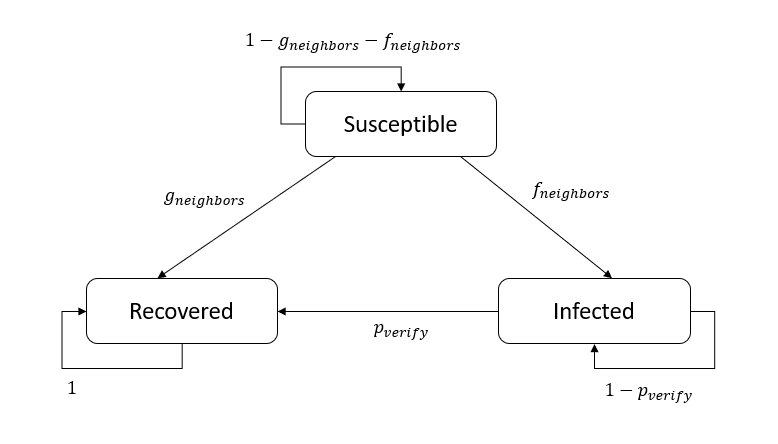
\includegraphics[scale=.9]{figs/Tambuscio_modified.png}
    \caption{state chart for the modified model}
    \label{modifiedmodelstatechart}
\end{figure}

\begin{table}[ht!]
    \centering
    \begin{tabular}{|c  c |} 
     \hline
     & \\
     $\begin{aligned}
          p_i^S(t+1) &= (1-f_i-g_i)s_i^S(t) \\
          p_i^I(t+1) &= f_is_i^S(t) + (1-p_{verify})s_i^I(t) \\
          p_i^R(t+1) &= g_is_i^S(t) + p_{verify}s_i^I(t)+s_i^R(t)
        \end{aligned}$
      &
      $\begin{aligned}
          f_i(t) &= \beta \frac{n_i^I(t)(1+\alpha)}{n_i^I(t)(1+\alpha)+n_i^R(t)(1-\alpha)} \\
          g_i(t) &= \beta \frac{n_i^R(t)(1-\alpha)}{n_i^I(t)(1+\alpha)+n_i^R(t)(1-\alpha)} \\
        \end{aligned}$
       \\ 
       & \\
     \hline
    \end{tabular}
    \caption{modified probability functions for the states}
    \label{modified-SIS-table-equations}
\end{table}

The propagation of the information in the proposed algorithm 
progresses after each iteration step $i$. The algorithm divides the 
information propagation process in two parts. In the first part, 
the probabilities $p_n(t+1) = [p_i^S, p_i^I, p_i^R]$ for all nodes are
calculated. Then, the states of all nodes are changed 
based on the probabilities calculated in the previous step.
By separating both steps, it can be ensured that state changes
in the current iteration cannot influence the calculation
of the probability $p_n(t+1)$ of the other nodes.


\subsection{Rule-based Calculation of the Power Consumption}
\label{rulebasedpowerconsumption}

Last, given the social network modeling components given in 
Sections \ref{simulationframeworksection} and 
\ref{modelinformationdiffusion}, the rules to model the
power demand changes need to be defined.
To model the demand changes in the simulation, multiple assumptions
are made.
First, it is assumed that only \textit{infected} entities in 
the social network graph
can change their power demand. The reason is 
that only changes in power demand due to social media information
are considered. Moreover, since \textit{susceptible} entities
do not know of the information being spread on social media and 
\textit{recovered} entities do not believe in the information anymore,
these entities do not act on the information, unlike infected
entities.
Next, it is assumed that every entity in the social network graph 
models one household, and not a person. There are 
two reasons for this assumption. First, it is assumed that 
members of a single household are highly connected and if one 
member of a household receives the information, all other members
will be informed as well. Next, it is simpler to model power demand
patterns on a household level than a person level. The reason
is that usually
there is one of each appliance that consume a lot of electricity, 
such as washing machines, ovens or dryers, in each household.
Then, it is assumed that the time of infection of an entity may not
coincide with the time where the entity changes its 
power consumption. This is due to the fact that in the information
being spread on social media, there may be be points in time
mentioned, thus leading to a delayed action response by the
infected entities. An example scenario that benefits
from these assumption is a false pricing information scenario 
mentioned in Section \ref{contextmotivation}, Chapter 
\ref{relatedworks} and Section \ref{demandresponsesection} 
In this assumption, an entity may receive the information 
at 3PM that the electricity price will be reduced 
between 5PM and 7PM. Thus, the household already received the
information and may be considered as infected in the social network
graph, but it will not act on the information since changing
its power demand would only benefit it starting 5PM. Thus, its 
action will be delayed until 5PM. 

Besides the these assumptions, other assumptions are made 
to provide more realistic simulation results. 
First, it is assumed that there may not be an immediate change 
in power demand even if an entity is both infected and the entity 
is in the time window to take action. This means that even if
both conditions are fulfilled, the entity may delay its action. 
Therefore, it is assumed that for each infected entity that can 
take action with the probability $p_{\mathrm{power\_usage}}$, where 
$p_{\mathrm{power\_usage}}$ is a system
parameter that defines the probability where an entity
starts changing its power demand when both other conditions are
fulfilled. Furthermore, this condition is continuously checked 
during the simulation until the condition is fulfilled.
Another assumption is that even if both conditions that
the entity is infected and the entity is in the time window 
to take action, the entity may not take action.
The idea is that even if an entity knows and believes
in the information that is being spread and may also spread
the information to its friends, it may not have the motivation to 
act on the information.
This assumption is given with the probability $p_{\mathrm{will\_act}}$.
This assumption, contrary to the former assumption, is only
checked once. If the condition is not fulfilled, the 
entity will never act on the information, even if 
it believes in the information. Last, it 
is also assumed that some entities may not be able to participate due 
to constraints that are outside of their control. For example, 
one entity may be interested in participating in energy reduction
program to reduce his energy costs, but is unable to do so since 
the entity has an energy provider which does not offer such a program.
Thus, even if the entity is infected and would like to act on the 
information, contextual contraints do not allow him to participate in it.
Nonetheless, the entity can still spread the information to its neighbors
which might be able to act on it. 
This availability to participate in the power demand change event is 
given with the probability $p_{\mathrm{available}}$.
Furthermore, there may be scenarios where 
an entity both does not act on the information and does not 
spread the information further. 

The power demand changes should be comparable to reference data.
For this, load profiles are used as reference points to increase
or reduce power demand from consuming entities. Load profiles
show the average power consumption behavior of consumers and 
are used by electricity providers to predict the power demand
\cite{proedrou2021comprehensive}.
The load profile used for this Thesis is the standard load profile
for households created by the German Federal Association of Energy and 
Water Management (Bundesverband der Energie- und Wasserwirtschaft 
e. V. (BDEW)) \cite{meier1999reprasentative}.
For each infected household, the additional power usage is 
added on top of the power demand given by the load profile.
The additional power usage is defined by the appliances in each
household that are of relevance for the specific scenario. 
The appliances and other system parameters are defined
in a JSON file. An example JSON file is shown in Listing 
\ref{appliancejsonfile}.

\begin{lstlisting}[language=json,firstnumber=1, 
    caption={Example parameters for household appliances for 
    the simulation},captionpos=b,label={appliancejsonfile}]
{
    "model_args":{
        "electric_car": {
        "power": 1125,
        "p": 0.1,
        "duration": 10000
        },
        "washing_machine": {
        "power": 100,
        "p": 95.8,
        "duration": 4
        }
    },
    "sim": {
        "p_will_act": 0.6,
        "p_power_usage": 0.8,
        "p_verify": 0.07,
        "alpha": 0.4,
        "beta": 0.6,
        "power_threshold": 1.5
        "factor": 1
    },
    "network":{
        "nodes": 400,
        "available": 0.9,
        "fringe": false
      }, 
}
\end{lstlisting}

Each appliance used in a specific scenario 
is defined in Listing \ref{appliancejsonfile} in the 
\code{model\_args} field. The definition of each 
appliance contains three parameters. The \code{power}
parameter defines by how much the power consumption
increases if the appliance is used in a household.
Next, the \code{p} parameter defines the probability that 
a specific household possesses the appliance. The reason for
this parameter is that not all households may possess
every household appliance defined in the JSON file.
Then, the \code{duration} parameter defines for which duration
$\Delta t$ the appliance is turned on an thus contributes
to the change in power consumption. Furthermore, in 
the \code{sim} and the \code{network} fields, 
multiple system and network parameters
necessary for the simulation and network 
model generation are defined.
The parameter \code{n} defines the size $N$ of the social media graph.
Next, the parameters \code{alpha}, \code{beta} and \code{p\_verify}
are used for the information propagation process.
Then, the parameters \code{p\_will\_act}, \code{p\_power\_usage}
ans \code{available}
were alread described in the assumptions. 
\code{fringe} is the parameter used to define if a specific scenario
is a fringe scenario, where unavailable entities do not share 
information even if they receive it.
Next, a critical threshold needs to be defined 
for when the power grid is overstressed by the 
total power consumption and a blackout occurs.
The critical threshold is defined as $a$ times
the maximum power consumption in the reference power
consumption data. The threshold factor can be seen
in the Listing \ref{appliancejsonfile} as the
\code{power\_threshold} parameter.

Given the assumptions and the system parameters, the simulation 
algorithm can thus be introduced. 
It is assumed that the the social network graph used in the algorithm
is initialized with each node belonging to the \textit{Susceptible} class. 
Then, in the initialization step of the simulation algorithm,
one node of the social network graph becomes infected,
thus acting as the initial source of information in the network.
Next, for each iteration step $i$, the total power demand 
based on the information in the social network is calculated.
The total power demand is calculated as the sum of the 
power consumption of all nodes in the network. 

\begin{equation}
    power_n=factor \cdot power_{ref}+offset
    \label{power-calc-equation}
\end{equation}

The equation to calculate the power consumption 
of a node $n$ if it is infected is shown in Equation \ref{power-calc-equation}. 
If the node is not infected, then the power consumption of the node 
equals the reference data $power_{ref}$, since it is 
not affected by the information and thus does not change it's
behaviour. Furthermore, Equation \ref{power-calc-equation} 
is only used if the date of current iteration $t_i$
is after the date where entities can act 
on the information being spread. Else, power consumption
equals to the reference data $power_{ref}$.
The variable $offset$ in Equation \ref{power-calc-equation} 
is the sum of all appliances defined in the JSON file (as shown in Listing 
\ref{appliancejsonfile}) that are used by the 
specific household whose time $\Delta t$ is still active.
Aditionally, the power usage can be 
scaled by the factor $factor$, which is a parameter defined in 
the \code{sim} field in the JSON file. 
After the calculation of the power usage, the information is 
propagated in the network graph. The algorithm 
for the information propagation step was defined in Section 
\ref{modelinformationdiffusion}.
After each iteration of the information propagation algorithm,
it is checked whether the infected individuals will act on 
the information. For this, it is first checked whether
the newly infected households will ever act on the information.
This constraint is calculated with the condition
$p<p_{\mathrm{will\_act}}$.
Next, it will check whether
an infected individual will delay its action, even if
all other constraints that hinder overconsumption of power
are fulfilled. This constraint is checked with the
condition $p<p_{\mathrm{power\_usage}}$. 
Then, it will start with the next iteration $i+1$.

Next, the main components of the simulation framework are shown
in Figure \ref{simframework}.
The simulation algorithm receives as input a social 
network graph, reference power consumption data with their 
corresponding dates and 
a JSON file with the simulation parameters. 
Then, the simulation algorithm is executed.
The algorithm is run over
$m$ steps. Next, the output of the simulation is the 
power demand over the time $[t, t+m]$ based on the
input parameters.

\begin{figure}[!ht]
    \center
    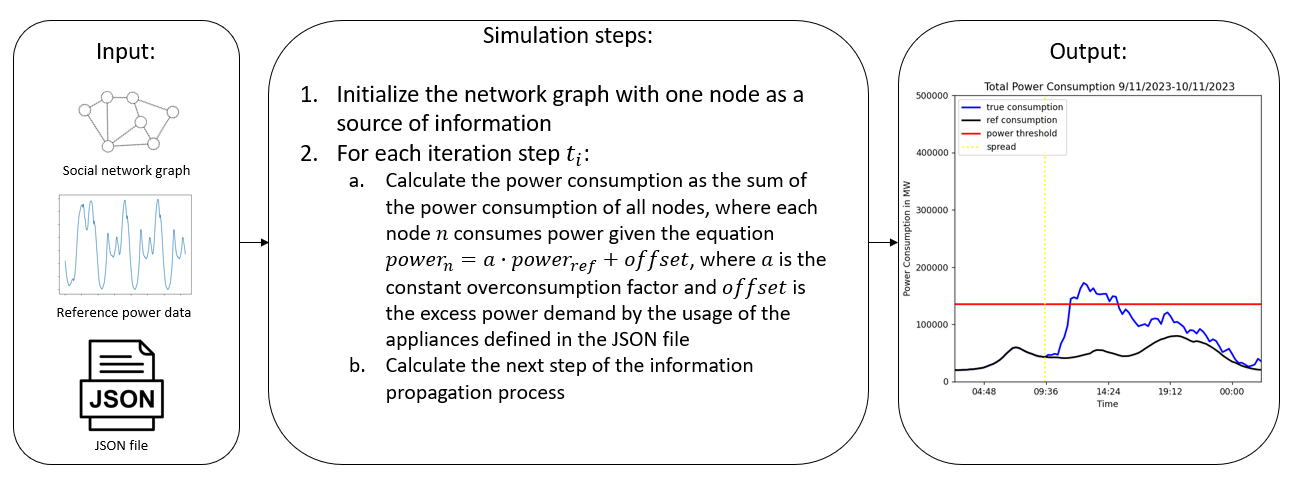
\includegraphics[scale=.66]{figs/Simulation-framework.png}
    \caption{Basic structure of the simulation framework}
    \label{simframework}
\end{figure}

The output can either be returned as a list with $m$ values
or an animation generated with the \textit{Matplotlib} package.
\textit{Matplotlib} is a Python package used to plot and visualize 
data. The animations are generated to show the information propagation
progress dynamically and show its real-time effects on the power
consumption curve. The simulation framework can generate two 
kinds of animations. Both are shown in Figure \ref{both-anim-views}.
One animation typeshown in Figure \ref{graph-view}
provides a graph-based view, which 
shows which nodes are at which state at an iteration step $i$.
The other animation type shown in Figure \ref{system-view}
provides a system-wide view, which shows
the changes in number of households belonging to each of the three
states over time.
The graph-based view can be used to analyze the information propagation
process for small models. For big models with a high number of nodes
in the social network graph, the graph-based view tends to be 
computationally expensive. Thus, the system-wide view should be used
for big models.


\begin{figure}[!ht]
    \begin{subfigure}{\textwidth}
    \centering
    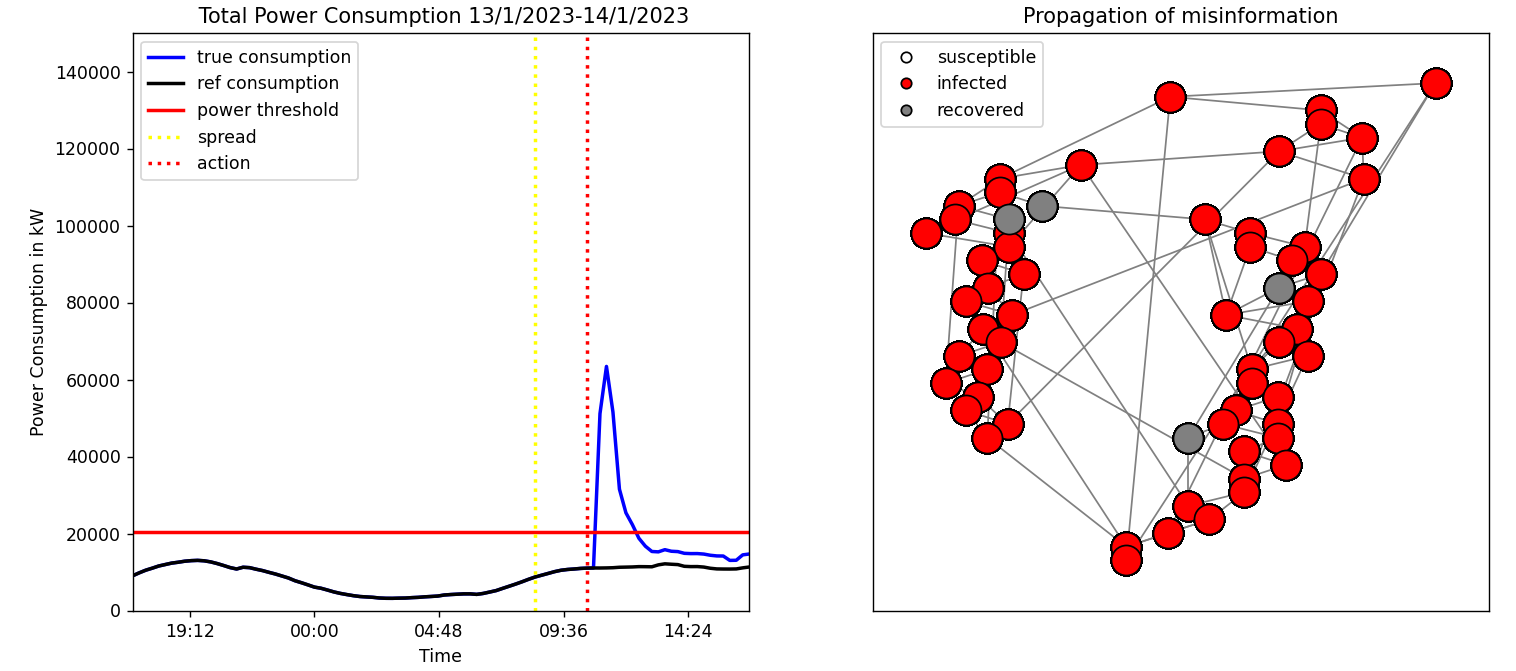
\includegraphics[scale=.5]{figs/graph-wide-view.png}
    \caption{graph-based view}
    \label{graph-view} 
    \end{subfigure}
    \begin{subfigure}{\textwidth}
    \centering
    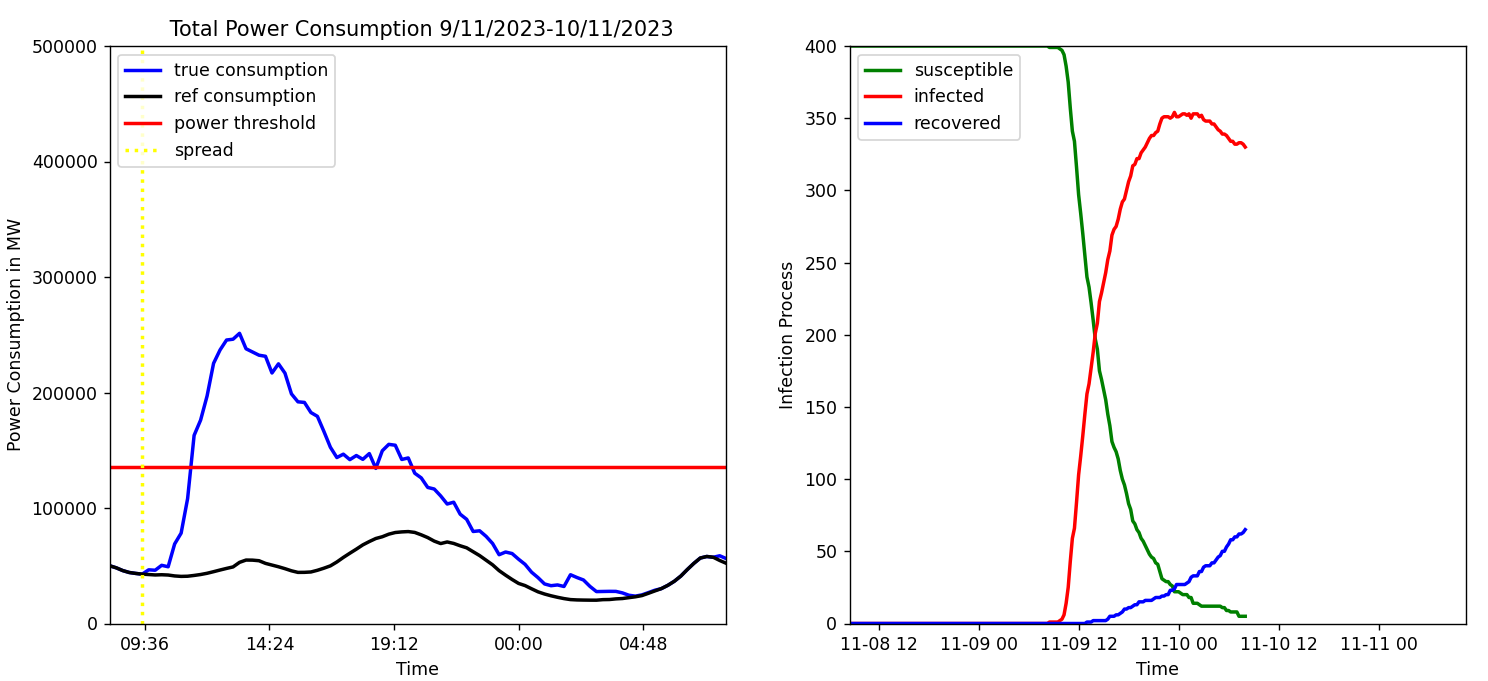
\includegraphics[scale=.505]{figs/system-wide-view.png}
    \caption{system-wide view}
    \label{system-view}
    \end{subfigure}
    \caption{Two different variations of the animations provided
    by the simulation framework}
    \label{both-anim-views}
\end{figure}



\section{Framework for System Parameter Estimation}
\label{parameterestimationalgo}

In Section \ref{simulationframeworksection}, a framework to simulate the effects 
of information on the power grid was introduced. However, the simulation results
may differ significantly based on which parameters were chosen for the simulation.
Furthermore, if the systems parameters are chosen without any real-life basis,
the result of the simulation may be unrealistic. Thus, the simulation framework 
may not be useful to predict possible crisis scenarios.
As a consequence, if the framework should produce realistic results and if
it should be used to possibly predict excess power consumption, an 
algorithm to estimate realistic values for the system parameters is necessary.

In Section \ref{powerloadsection}, different variables that 
correlate with power load were introduced. These variables can be 
used to estimate realistic system parameters. For this Thesis, social media data is 
used to estimate the system parameters that control the 
information propagation. Since it is difficult to get personalized 
information of people on the internet due of data privacy reasons, the
social media data is assumed to be as generalized as possible. Moreover, the identity 
of the users posting messages is assumed to be unknown. The only information
that is being considered in this Thesis are the number of messages in a given timespan.
One method to estimate the propagation parameters of the SIR model 
is to view the problem as a minimization problem 
\cite{jin2013epidemiological}. The idea is to iteratively solve the differential 
equations of the SIR model, analyze the infection process and minimize 
its difference of the true infection process that can be seen via the
social media data. A simplified diagram with the steps of the algorithm
can be seen in Figure \ref{paramestimationbasic}. The method proposed 
in this Thesis contains five different steps. 
The first three steps are used to gather and preprocess 
the data that is of relevance for the parameter estimation process.
The last two steps make up the parameter estimation algorithm.
The steps in the proposed method are:

\begin{enumerate}
    \item Find all relevant posts and messages on social media websites.
    This can be done either with natural language processing techniques or
    by using keyword search queries.
    \item Count the number of relevant social media posts over a given 
    timespan. This is done by counting the number of posts in given intervals, 
    such as e.g. the number of posts each 15 minutes. This data shows the
    engagement on the specific topic over time.
    \item Filter the data graph to smoothen the data and to facilitate the
    parameter extraction process. The filtered data is $posts(t)$.
    \item Initialize the minimization algorithm with predefined unknown
    variables and their initial values. Optimize the variables
    so that the difference of the curve progression of the SIR model
    and the number of posts over time is minimized. For each minimization
    step, the differential equations that define the infection progression
    in the system need to be solved.
\end{enumerate}

\begin{figure}[!ht]
    \center
    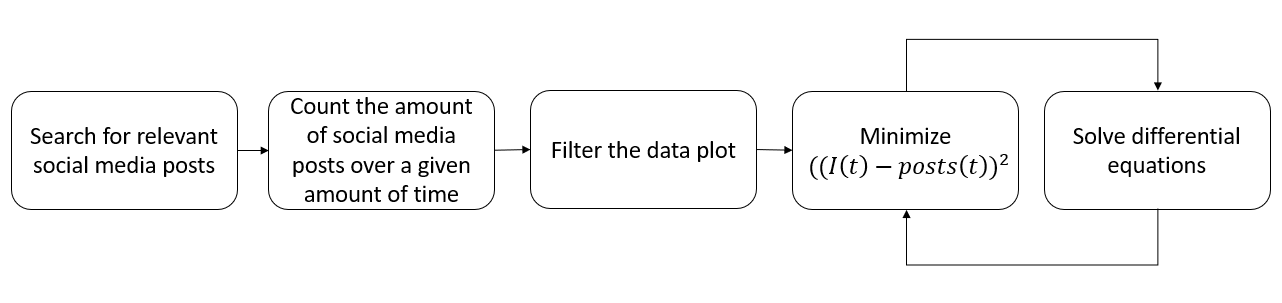
\includegraphics[scale=.65]{figs/parameter_estimation_process.png}
    \caption{Steps of the parameter estimation algorithm}
    \label{paramestimationbasic}
\end{figure}

To use the algorithm proposed in this Thesis, it is necessary to 
know the specific differential equations that describe the propagation 
process over time. However, the propagation algorithm
used in the simulation framework is not based on differential equations,
but is a graph-based algorithm. Since it is graph-based, the propagation algorithm
does not provide a system-wide view on the propagation process.
It considers the local status of the infection, i.e the neighbors
of each node, to decide on the state of a specific node.
To calculate the differential equations for the specific SIR model algorithm
used in this Thesis, mean-field theory is used to generalize the equations
\cite{chaikin1995principles}.
This is done by averaging certain variables in the system, making these
variables constant over the model and thus 
reducing the degrees of freedom that need to be considered.
Thus, all unique interactions in the model are averaged into a simpler,
higher-level or system-wide view.
This approach originated from molecular analysis, where the method is used
to average the behaviors of many molecules into the average behavior
of the whole system,
but it can also be used to analyze the characteristics of graphs
\cite{barabasi1999mean}\cite{sirsmodel}.
Thus, mean-field theory is used in this Thesis to 
analyze the average interactions in the graph and thus to deduce 
the average characteristics of the information 
propagation process. 

To analyze the average information propagation process, 
it can be assumed that for a Barabási–Albert random graph, 
the median degree for a node in the graph will be equal to the number 
of edges generated when adding a new node to the random graph.
This assumption can be made since the graph follows the power law distribution,
which defines that few nodes have a high amount of connections to other nodes
and a high number of nodes have comparatively low number of connections to 
other nodes. Since the minimum number of edges that a node can have 
in the Barabási–Albert random graph generation algorithm is $k$, this 
means that we can assume that $\forall i \to c_i=k$.
Next, we define the parameters $S(t), I(t), R(t)$, where $S(t)$ is the number of
entities in the system with the status \textit{Susceptible} at the time $t$, 
$I(t)$ is the number of entities with the status \textit{Infected} and
$R(t)$ is the number of entities with the status \textit{Recovered}. 
We assume that the states of the neighbors of a node $i$ at the time $t$ are 
randomly distributed given the probabilities $p^S(t), p^I(t), p^R(t)$,
where $p^S(t) + p^I(t) + p^R(t) = 1$. We can calculate the values $S(t), I(t), R(t)$
with the Equations in \ref{SIR-system-amound-eqs:all-lines},
with $N$ as the total number of entities in the system.

\begin{subequations}
\begin{align}
    S(t) &=p^S(t)\cdot N \label{SIR-system-amound-eqs:1}\\
    I(t) &=p^I(t)\cdot N \label{SIR-system-amound-eqs:2}\\
    R(t) &=p^R(t)\cdot N \label{SIR-system-amound-eqs:3}
\end{align}
\label{SIR-system-amound-eqs:all-lines}
\end{subequations}

Given the Equations in \ref{SIR-system-amound-eqs:all-lines}, it is possible 
to calculate the changes $\Delta S(t), \Delta I(t), \Delta R(t)$ between each 
iteration step $t$ and $t+1$ in the system.
The changes can be calculated with the Equations defined in 
\ref{SIR-diff-system-amount-eqs}.

\begin{subequations}
\begin{align}
    \frac{dS}{dt} \approx \frac{\Delta S(t)}{\Delta t} = \frac{\Delta S(t)}{1} = \Delta S(t) &=\Delta p^S(t)\cdot N \label{SIR-diff-system-amount-eqs:1}\\
    \frac{dI}{dt} \approx \frac{\Delta I(t)}{\Delta t} = \frac{\Delta I(t)}{1} = \Delta I(t) &=\Delta p^I(t)\cdot N \label{SIR-diff-system-amount-eqs:2}\\
    \frac{dR}{dt} \approx \frac{\Delta R(t)}{\Delta t} = \frac{\Delta R(t)}{1} = \Delta R(t) &=\Delta p^R(t)\cdot N \label{SIR-diff-system-amount-eqs:3}
\end{align}
\label{SIR-diff-system-amount-eqs}
\end{subequations}

Since we assume that the states are randomly distributed over the model, 
we assume that the state of the node $i$ is randomly distributed.
Thus, the state $s_i$ of the node $i$ can be defined as in Equation 
\ref{state-node-equation}.

\begin{equation}
    s_i = [s_i^S, s_i^I, s_i^R] = [p^S(t), p^I(t), p^R(t)]
    \label{state-node-equation}
\end{equation}

Furthermore, the functions $g_i,f_i$ defined in Table 
\ref{modified-SIS-table-equations}
can be generalized by assuming that the average number of neighbors 
of a specific state $K$ can be calculated as $k\cdot p^K(t)$. For this
assumption, $k$ is the median degree of all nodes and $p^K(t)$ is the 
average probability that a node is in the state $K$.
Thus, the functions $g_i,f_i$ can be generalized as in
Equations \ref{generalized-functions-g-f}.

\begin{subequations}
\begin{align}
    f_i(t) &= \beta \frac{n_i^I(t)(1+\alpha)}{n_i^I(t)(1+\alpha)+n_i^R(t)(1-\alpha)} 
    \nonumber\\
    \to f(t) &= k\beta \frac{p^I(t)(1+\alpha)}{p^I(t)(1+\alpha)+p^R(t)(1-\alpha)}
    \label{generalized-function-f} \\
    g_i(t) &= \beta \frac{n_i^R(t)(1-\alpha)}{n_i^I(t)(1+\alpha)+n_i^R(t)(1-\alpha)} 
    \nonumber \\
    \to g(t) &= k\beta \frac{p^R(t)(1-\alpha)}{p^I(t)(1+\alpha)+p^R(t)(1-\alpha)}
    \label{generalized-function-g}
\end{align}
\label{generalized-functions-g-f}
\end{subequations}

With these assumptions, the general equations for the SIR model can 
be deduced. First, the function for $\Delta R(t)$ can be infered
as shown in Equation \ref{delta-r-deduction-eqs}.

\begin{align}
    p^R(t+1) &= g \cdot p^S(t) + p_{verify}\cdot p^I(t) + p^R(t) \nonumber\\
    p^R(t+1) - p^R(t) &= g \cdot p^S(t) + p_{verify}\cdot p^I(t) \nonumber\\
    \Delta R(t) = (p^R(t+1) - p^R(t))\cdot N 
    &= N(g \cdot p^S(t) + p_{verify}\cdot p^I(t)) \nonumber\\
    &= N(g \cdot \frac{S(t)}{N} + p_{verify}\cdot \frac{I(t)}{N} ) \nonumber\\
    &= g \cdot S(t) + p_{verify}\cdot I(t) \nonumber\\
    &= k\beta \frac{p^R(t)(1-\alpha)}{p^I(t)(1+\alpha)+p^R(t)(1-\alpha)} 
    \cdot S(t) + p_{verify}\cdot I(t) \nonumber\\
    &= k\beta \frac{\frac{R(t)}{N}(1-\alpha)}{\frac{I(t)}{N}(1+\alpha)+\frac{R(t)}{N}(1-\alpha)} 
    \cdot S(t) + p_{verify}\cdot I(t) \nonumber\\
    \Delta R(t) &= \frac{k\beta}{N} \frac{R(t)(1-\alpha)}{I(t)(1+\alpha)+R(t)(1-\alpha)} 
    \cdot S(t) + p_{verify}\cdot I(t) \label{delta-r-deduction-eqs}
\end{align}

The equation for $\Delta I(t)$ can be infered in a similar manner to $\Delta R(t)$.
The deduction steps for $\Delta I(t)$ are shown in Equation 
\ref{delta-i-deduction-eqs}.

\begin{align}
    p^I(t+1) &= f \cdot p^S(t) + (1 - p_{verify})\cdot p^I(t) \nonumber\\
     &= f \cdot p^S(t) + p^I(t) - p_{verify}\cdot p^I(t) \nonumber\\
    p^I(t+1) - p^I(t) &= f \cdot p^S(t) - p_{verify}\cdot p^I(t) \nonumber\\
    \Delta I(t) = (p^I(t+1) - p^I(t)) \cdot N 
    &= N (f \cdot p^S(t) - p_{verify}\cdot p^I(t)) \nonumber\\
    &= N (f \cdot \frac{S(t)}{N}  - p_{verify}\cdot \frac{I(t)}{N}) \nonumber\\
    &= f \cdot S(t) - p_{verify}\cdot I(t) \nonumber\\
    &=  k\beta \frac{p^I(t)(1+\alpha)}{p^I(t)(1+\alpha)+p^R(t)(1-\alpha)}
     \cdot S(t) - p_{verify}\cdot I(t) \nonumber\\
    &=  k\beta \frac{\frac{B(t)}{N}(1+\alpha)}{\frac{I(t)}{N}(1+\alpha)+\frac{R(t)}{N}(1-\alpha)}
     \cdot S(t) - p_{verify}\cdot I(t) \nonumber\\
     \Delta I(t) &=  \frac{k\beta}{N} \frac{I(t)(1+\alpha)}{I(t)(1+\alpha)+R(t)(1-\alpha)}
     \cdot S(t) - p_{verify}\cdot I(t) \label{delta-i-deduction-eqs}
\end{align}

Last, given that there are no entities entering or leaving the system,
it can be assumed that the state changes in the system all sum to zero,
thus $\Delta S(t)+ \Delta I(t)+ \Delta R(t) = 0$. With this, the equation for
$\Delta S$ can be deduced as shown in Equation \ref{delta-s-deduction-eqs}.

\begin{align}
    \Delta S(t) &= - \Delta I(t) - \Delta R(t) \nonumber\\
     &= -\frac{k\beta}{N} \frac{I(t)(1+\alpha)}{B(t)(1+\alpha)+R(t)(1-\alpha)}
     \cdot S(t) + p_{verify}\cdot I(t) \nonumber\\
      & -\frac{k\beta}{N} \frac{R(t)(1-\alpha)}{B(t)(1+\alpha)+R(t)(1-\alpha)} 
      \cdot S(t) - p_{verify}\cdot I(t) \nonumber\\
      &= -\frac{k\beta}{N} \frac{I(t)(1+\alpha) + R(t)(1-\alpha)}{I(t)(1+\alpha)+R(t)(1-\alpha)}
      \cdot S(t) + p_{verify}\cdot I(t) - p_{verify}\cdot I(t) \nonumber\\
      &= -\frac{k\beta}{N} \frac{I(t)(1+\alpha) + R(t)(1-\alpha)}{I(t)(1+\alpha)+R(t)(1-\alpha)}
      \cdot S(t) \nonumber\\
      \Delta S(t) &= -\frac{k\beta}{N} \cdot S(t) \label{delta-s-deduction-eqs}
\end{align}


Summarized, the differential equations that are used for the parameter estimation 
algorithm can be seen in Equation \ref{all-deduced-diff-equations}.

\begin{subequations}
    \begin{align}
        \frac{dS}{dt} \approx \Delta S(t) &= -\frac{k\beta}{N} \cdot S(t) \\
        \frac{dI}{dt} \approx \Delta I(t) &=  \frac{k\beta}{N} \frac{I(t)(1+\alpha)}{I(t)(1+\alpha)+R(t)(1-\alpha)}
        \cdot S(t) - p_{verify}\cdot I(t) \\
        \frac{dR}{dt} \approx \Delta R(t) &= \frac{k\beta}{N} \frac{R(t)(1-\alpha)}{I(t)(1+\alpha)+R(t)(1-\alpha)} 
        \cdot S(t) + p_{verify}\cdot I(t)
\end{align}
\label{all-deduced-diff-equations}
\end{subequations}


The differential equations have multiple unknown variables that need
to be optimized in the minimization process. One unknown variable is
the true size of the system $N$ since $N$ does not need to correlate 
with the size of the social media website $N_{website}$.
Another unknown variable is the average degree $k$ of the social network,
since we do not know the specific characteristics of the network of the
subgroup infected or susceptible to the information.
Next, the three propagation parameters $\alpha, \beta, p_{verify}$ are not known
and need to be optimized. 
Last, the initial values $S(t_0), I(t_0), R(t_0)$ are also not known.
Thus, there are seven variables $N, k, \alpha, \beta, p_{verify}, 
S(t_0), I(t_0), R(t_0)$
that need to be optimized.


Next, in conjunction with the simulation framework described in 
\ref{simulationframeworksection}, it should be possible to predict 
a possible overconsumption scenario. For this, a framework
to predict power demand surges started by information shared in 
social media networks is proposed in this Thesis. The steps
in the proposed framework are shown in Figure \ref{basicpredicitonframework}.
First, the data used for the parameter estimation process is gathered and
preprocessed. Then, this data is used for the parameter estimation algorithm. 
Afterwards, the simulation framework is configured
with the parameter estimated in the previous step. For this, 
$\alpha, \beta, p_{verify}, S(t_0), I(t_0), R(t_0)$ are used to configure the 
information propagation process implemented in the simulation framework.
The variables $N$ and $k$ are used to configure the random graph generation
characteristics. The implementation of the 
algorithm of the Barabási–Albert random graph in \textit{NetworkX}
receives the total number of nodes in the graph and the number of edges 
for each incoming node as inputs. Since we assume that the median degree
$k$ equals the number of edges generated for each incoming node, we can thus
use $k$ as an input for the random graph algorithm. However, this assumption
only works if the total number of nodes in the random graph is $N$.
Since social networks tend to be big, it can be assumed that 
$N$ is of high value and that a graph of such a size may lead to technical 
issues such as high computation time. Thus, smaller values such as $N'$
can be used as long as the ration between the number of nodes and the
number of edges for the incoming nodes are the same, thus the constraint
$\frac{k}{N}=\frac{k'}{N'}$ needs to be fulfilled for a Barabási–Albert
graph $G'(N',k')$. With the parameters for the information propagation and 
for the random graph, the simulation can thus be run. 
Last, given the results of the simulation and the power threshold
that define the upper limit of the power grid infrastructure, it
is checked whether the power demand exceeds the predefined threshold.


\begin{figure}[!ht]
    \center
    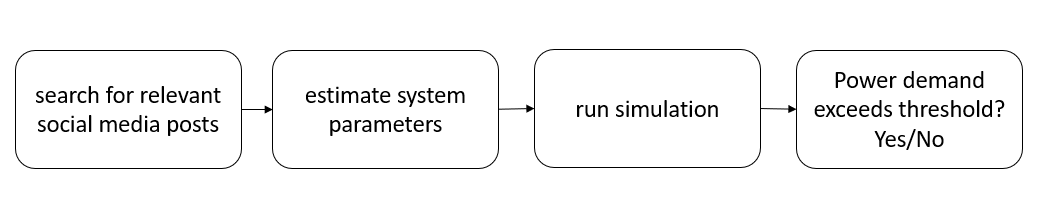
\includegraphics[scale=.65]{figs/full_prediction_framework.png}
    \caption{Steps of the proposed framework to predict power demand surges
    started by information shared in social media networks}
    \label{basicpredicitonframework}
\end{figure}


% als letzte Idee: herleiten, ab welchen p_verify I_max unter 
% ein bestimmtes threshhold ist